\documentclass[aspectratio=169]{beamer}

\usetheme{default}
\usecolortheme{default}
\useinnertheme{rectangles}
\setbeamertemplate{navigation symbols}{}

\usepackage[T1]{fontenc}
\usepackage[utf8]{inputenc}
\usepackage{lmodern}
\usepackage{hyperref}
\usepackage[numbers]{natbib}
\usepackage{tikz}

\definecolor{arbg}{HTML}{F6F8FB}
\definecolor{artext}{HTML}{1F2933}
\definecolor{arblue}{HTML}{204B76}
\definecolor{arteal}{HTML}{2C7A7B}
\definecolor{araccent}{HTML}{D9A441}

\setbeamercolor{background canvas}{bg=arbg}
\setbeamercolor{normal text}{fg=artext,bg=arbg}
\setbeamercolor{structure}{fg=arblue}
\setbeamercolor{frametitle}{fg=white,bg=arblue}
\setbeamercolor{title}{fg=white}
\setbeamercolor{subtitle}{fg=arbg}
\setbeamercolor{author}{fg=artext}
\setbeamercolor{date}{fg=artext}
\setbeamercolor{block title}{fg=white,bg=arteal}
\setbeamercolor{block body}{fg=artext,bg=white}
\setbeamercolor{footline}{fg=arbg,bg=arblue}
\setbeamercolor{item projected}{fg=white,bg=arteal}

\setbeamerfont{title}{series=\bfseries,size=\LARGE}
\setbeamerfont{subtitle}{size=\large}
\setbeamerfont{frametitle}{series=\bfseries,size=\large}
\setbeamerfont{block title}{series=\bfseries}

\setbeamertemplate{itemize item}{\color{arteal}\large\textbullet}
\setbeamertemplate{itemize subitem}{\color{araccent}\normalsize\textbullet}
\setbeamertemplate{blocks}[rounded][shadow=false]

\setbeamertemplate{title page}{
  \vspace*{0.08\paperheight}
  \begin{center}
  \begin{beamercolorbox}[wd=0.9\paperwidth,sep=1.2em,rounded=true,shadow=false]{frametitle}
    {\raggedright\usebeamerfont{title}\inserttitle\par}
    \vspace{0.35em}
    {\raggedright\usebeamerfont{subtitle}\insertsubtitle\par}
  \end{beamercolorbox}
  \end{center}

  \vspace{1.5em}
  {\color{araccent}\rule{0.22\paperwidth}{1.5pt}}

  \vfill

  \begin{flushleft}
    {\usebeamerfont{author}\insertauthor\par}
    \vspace{0.35em}
    {\usebeamerfont{date}\insertdate\par}
  \end{flushleft}
}

\setbeamertemplate{footline}{
  \leavevmode
  \hbox{
    \hspace*{0.02\paperwidth}
    \begin{beamercolorbox}[wd=0.96\paperwidth,ht=2.8ex,dp=1.2ex,leftskip=0.8em,rightskip=0.8em]{footline}
      \insertshorttitle\hfill\insertframenumber
    \end{beamercolorbox}
  }
}

\title{Autoresearch}
\subtitle{Autonomous Research and Software Development with LLM Agents}
\author{Ian Turner}
\date{\today}

\begin{document}

\begin{frame}
  \titlepage
\end{frame}

\begin{frame}{Table of Contents}
  \tableofcontents
\end{frame}

\section{What Is Autoresearch?}

\begin{frame}{What Is Autoresearch?}
  \centering
  \Large What Is Autoresearch?
\end{frame}

\begin{frame}{What Is Autoresearch?}
  \begin{itemize}
    \item Using AI agents to automate the \textbf{research process itself}
    \item Distinct from AI applied to a domain problem (medical diagnosis, protein folding, image generation)
    \item The agent generates ideas, designs and runs experiments, writes papers
    \item This talk: survey the current landscape --- systems, techniques, and limitations
  \end{itemize}
\end{frame}

\begin{frame}{The Spectrum of AI-Assisted Research}
  \vspace{2em}
  \begin{center}
  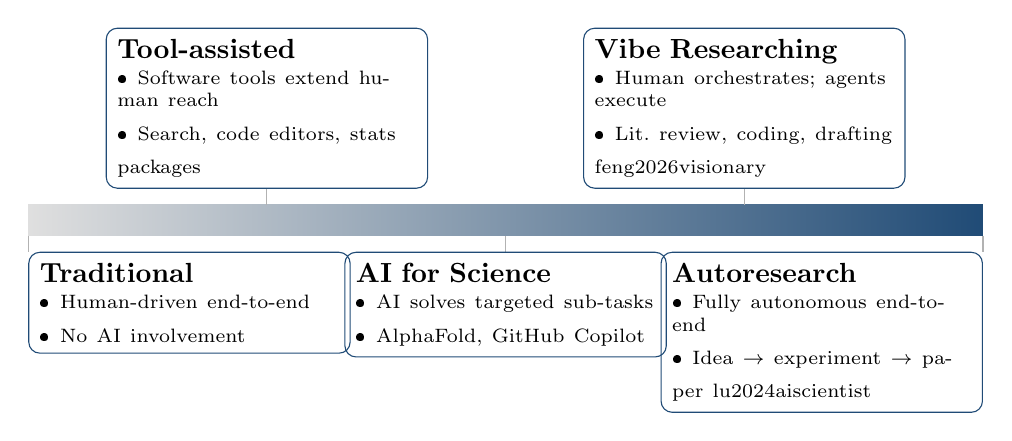
\begin{tikzpicture}[x=\linewidth, y=1cm]
    \shade[left color=gray!25, right color=arblue]
      (0, 0) rectangle (1, 0.4);

    % Above: Tool-assisted, Vibe Researching
    \draw[gray!60] (0.25, 0.4) -- (0.25, 0.6);
    \draw[gray!60] (0.75, 0.4) -- (0.75, 0.6);
    \node[above, align=left, text width=3.8cm, draw=arblue, rounded corners, inner sep=4pt] at (0.25, 0.6) {
      \textbf{Tool-assisted}\\[0.15em]
      \scriptsize\textbullet\ Software tools extend human reach\\
      \textbullet\ Search, code editors, stats packages
    };
    \node[above, align=left, text width=3.8cm, draw=arblue, rounded corners, inner sep=4pt] at (0.75, 0.6) {
      \textbf{Vibe Researching}\\[0.15em]
      \scriptsize\textbullet\ Human orchestrates; agents execute\\
      \textbullet\ Lit.\ review, coding, drafting \citep{feng2026visionary}
    };

    % Below: Traditional, AI for Science, Autoresearch
    \draw[gray!60] (0,   0) -- (0,   -0.2);
    \draw[gray!60] (0.5, 0) -- (0.5, -0.2);
    \draw[gray!60] (1.0, 0) -- (1.0, -0.2);
    \node[below, align=left, text width=3.8cm, draw=arblue, rounded corners, inner sep=4pt, anchor=north west] at (0, -0.2) {
      \textbf{Traditional}\\[0.15em]
      \scriptsize\textbullet\ Human-driven end-to-end\\
      \textbullet\ No AI involvement
    };
    \node[below, align=left, text width=3.8cm, draw=arblue, rounded corners, inner sep=4pt] at (0.5, -0.2) {
      \textbf{AI for Science}\\[0.15em]
      \scriptsize\textbullet\ AI solves targeted sub-tasks\\
      \textbullet\ AlphaFold, GitHub Copilot
    };
    \node[below, align=left, text width=3.8cm, draw=arblue, rounded corners, inner sep=4pt, anchor=north east] at (1.0, -0.2) {
      \textbf{Autoresearch}\\[0.15em]
      \scriptsize\textbullet\ Fully autonomous end-to-end\\
      \textbullet\ Idea $\to$ experiment $\to$ paper \citep{lu2024aiscientist}
    };
  \end{tikzpicture}
  \end{center}
\end{frame}

\section{The Research Pipeline}

\begin{frame}{The Research Pipeline}
  \centering
  \Large The Research Pipeline
\end{frame}

\begin{frame}{The Research Lifecycle}
  \begin{enumerate}
    \item Idea Generation \& Literature Review
    \item Research Planning \& Experiment Design
    \item Data Preparation \& Experiment Execution
    \item Results Analysis
    \item Report Writing \& Synthesis
    \item Paper Review
  \end{enumerate}
  \vfill
  \footnotesize\textit{Literature review is the most consistently failing stage across current systems.} \citep{schmidgall2025agenticscience}
\end{frame}

\begin{frame}{Stage 1: Idea Generation}
  \begin{itemize}
    \item LLM brainstorms ideas from a research prompt or template
    \item \textbf{Novelty filtering}: Semantic Scholar API rejects ideas too similar to existing work
    \item \textbf{Scoring rubric}: each idea rated 1--10 on Interestingness, Feasibility, and Novelty
    \item Multiple rounds of \textbf{chain-of-thought + self-reflection} refine and diversify the idea set
    \item A running archive prevents re-proposing already-explored ideas
  \end{itemize}
  \vfill
  \footnotesize\citep{lu2024aiscientist}
\end{frame}

\begin{frame}{Stage 2: Experimentation}
  \begin{itemize}
    \item \textbf{Aider} (LLM coding agent) implements plan-directed code changes; runs experiments automatically
    \item \textbf{v1 (AI Scientist)}: linear loop --- implement $\to$ run $\to$ analyze $\to$ re-plan, up to 5 iterations
    \item \textbf{v2 (AI Scientist-v2)}: tree search --- parallel branches, best-first selection guided by an LLM evaluator; VLM checks generated figures
    \item Model comparison on v1 (best $\to$ worst): Claude Sonnet 3.5, GPT-4o, DeepSeek Coder (\textasciitilde\$10 total), Llama-3.1 405B
  \end{itemize}
  \vfill
  \footnotesize\citep{lu2024aiscientist, yamada2025aiscientistv2}
\end{frame}

\begin{frame}{Stage 3: Paper Writing \& Review}
  \begin{itemize}
    \item Paper written \textbf{section-by-section} by the LLM; LaTeX errors fed back for automated fixing
    \item \textbf{Semantic Scholar API} retrieves references for the related work section
    \item \textbf{Automated peer review}: GPT-4o reviewer with 5-round self-reflection and 5 ensembled reviews
    \item Reviewer accuracy: \textbf{70\% accept/reject} vs.\ 66\% for human reviewers \citep{lu2024aiscientist}
    \item Cost: \textbf{\$0.25--\$0.50 per review}; \textbf{\$15 per full paper}
    \item Milestone: first AI-generated paper accepted at a peer-reviewed venue (ICLR 2025 workshop, 1 of 3 submissions) \citep{yamada2025aiscientistv2}
  \end{itemize}
\end{frame}

\section{Case Studies}

\begin{frame}{Case Studies}
  \centering
  \Large Case Studies
\end{frame}

\section{Limitations and Risks}

\begin{frame}{Limitations and Risks}
  \centering
  \Large Limitations and Risks
\end{frame}

\section{Conclusions}

\begin{frame}{Conclusions}
  \centering
  \Large Conclusions
\end{frame}

\begin{frame}[allowframebreaks]{References}
  \footnotesize
  \nocite{*}
  \bibliographystyle{plainnat}
  \bibliography{references}
\end{frame}

\end{document}
